\documentclass[11pt,a4paper]{article}

% ---------------------------------------------------------------------------
% Preamble
% ---------------------------------------------------------------------------
\usepackage[margin=1in]{geometry}
\usepackage{amsmath,amssymb,amsthm}
\usepackage{graphicx}
\usepackage{booktabs}
\usepackage{listings}
\usepackage{xcolor}
\usepackage{hyperref}
\usepackage{algorithm}
\usepackage{algorithmic}
\usepackage{tikz}
\usepackage{array}
\usepackage{enumitem}
\usepackage{setspace}
\usepackage{caption}
\usepackage{microtype}
\usepackage{titlesec}

\usetikzlibrary{arrows.meta,positioning}

\hypersetup{
  colorlinks=true,
  linkcolor=blue!50!black,
  citecolor=blue!50!black,
  urlcolor=blue!60!black,
  pdftitle={Asclepius Clinical: Offline-First Voice-to-Prescription on the Edge},
  pdfauthor={Swayamsiddha}
}

\definecolor{codebg}{RGB}{248,249,252}
\definecolor{codekw}{RGB}{31,56,128}
\definecolor{codestr}{RGB}{163,21,21}
\definecolor{codecmt}{RGB}{0,110,40}
\definecolor{codeid}{RGB}{121,94,38}

\lstset{
  language=Python,
  basicstyle=\ttfamily\footnotesize,
  keywordstyle=\color{codekw}\bfseries,
  stringstyle=\color{codestr},
  commentstyle=\color{codecmt}\itshape,
  identifierstyle=\color{codeid},
  backgroundcolor=\color{codebg},
  frame=single,
  rulecolor=\color{black!20},
  breaklines=true,
  breakatwhitespace=false,
  showstringspaces=false,
  tabsize=4,
  columns=fullflexible,
  keepspaces=true,
  captionpos=b,
  numbers=left,
  numberstyle=\tiny\color{black!50},
  xleftmargin=2em,
  framexleftmargin=1.5em
}

\titleformat{\section}{\large\bfseries}{\thesection}{0.8em}{}
\titleformat{\subsection}{\normalsize\bfseries}{\thesubsection}{0.8em}{}
\setstretch{1.12}
\setlength{\parskip}{0.35em}

\title{\textbf{Asclepius Clinical: An Offline-First, Edge-Deployable\\
Voice-to-Prescription Assistant Combining Clinical ASR Priming,\\
Phonetic Drug Normalization, and Local LLM Entity Refinement}}

\author{Swayamsiddha\\
\textit{Student Researcher}\\
Doctor Voice-to-Prescription System (\texttt{Emb\_2})}
\date{11 October 2026}

\begin{document}
\maketitle

% ===========================================================================
\begin{abstract}
Spoken clinical consultations remain poorly served by cloud-centric electronic health record (EHR) tools: rural and bedside settings often lack reliable connectivity, while generic automatic speech recognition (ASR) systems distort Indian brand names, Latin dosing abbreviations, and pharmacology vocabulary. This report describes \textbf{Asclepius Clinical}, a local-first Flask application that converts a doctor's speech into a structured, reviewable prescription draft without requiring the internet at inference time. The pipeline captures audio from a microphone, system loopback, or file upload; applies DC-offset removal, Butterworth bandpass filtering, and RMS loudness normalization; transcribes with faster-whisper (CTranslate2 \texttt{int8}) primed by a clinical initial prompt; cleans ASR artefacts; extracts entities with a hybrid dictionary--regex engine; normalizes drugs via Soundex, a medical phonetic encoder, and sequence-ratio fuzzy matching against a $\sim$487-entry Indian formulary; optionally refines JSON with a quantized on-device LLM (Qwen2.5 1.5B / Llama~3.2 1B Medical / Qwen2.5 3B Medical); and validates the draft with a clinical decision-support rule engine. A 50-case specialty benchmark reports 87.7\% medication recall, 96.0\% diagnosis hit rate, and 9.55\,s mean refinement latency. The system is an assistive drafting tool: no prescription is finalized without explicit clinician confirmation.
\end{abstract}

\noindent\textbf{Keywords:}
clinical automatic speech recognition;
voice-to-prescription;
phonetic drug normalization;
edge LLM (GGUF);
clinical decision support;
offline-first EHR.

% ===========================================================================
\section{Introduction}

\subsection{Problem statement}
In high-throughput outpatient practice, especially in Indian primary and specialty clinics, a physician typically dictates diagnoses, brand-name medicines, frequencies such as ``1-0-1'' or ``BD'', and follow-up instructions while simultaneously examining the patient. Manual transcription into an EHR is slow and error-prone. Cloud speech APIs raise privacy, latency, and availability concerns for protected health information. Commodity ASR further fails in characteristic ways: Whisper splits brand names (``augment in''), verbalizes numbers (``five hundred milligrams''), and hallucinates common English words as drug names. The engineering problem is therefore to build an \emph{assistive}, \emph{offline-capable}, \emph{clinician-in-the-loop} pipeline that (i)~captures consultation audio on commodity hardware including Raspberry~Pi~5, (ii)~recovers a medically faithful transcript, (iii)~maps speech to a canonical prescription object, and (iv)~never silently finalizes therapy.

\subsection{Motivation}
The existing prototype in this workspace evolved from a three-mode Whisper transcriber (microphone, system audio, file upload) into a modular clinical assistant. Product intent, documented in \texttt{Plan.md}, is explicit: the software drafts; the doctor reviews, edits, and confirms. Local SQLite storage and an outbox table support opportunistic later synchronization. Edge constraints---CPU-only inference, $\sim$800\,MB--2.2\,GB LLM RAM budgets, Bluetooth HSP/HFP microphones on PipeWire---shape every design choice from \texttt{int8} ASR to greedy LLM decoding.

\subsection{Technical contributions}
The implemented system contributes the following:
\begin{itemize}[leftmargin=1.4em]
  \item A modular audio--ASR--NLP--prescription pipeline orchestrated by \texttt{app.py}, preserving three capture modes while adding consultation, patient, doctor, and PDF APIs.
  \item Clinical ASR priming (\texttt{CLINICAL\_INITIAL\_PROMPT} in \texttt{asr/whisper\_engine.py}) and a five-stage transcript cleaner (\texttt{clinical/transcript\_cleaner.py}) that map spoken numbers, units, frequencies, and split brand names onto extractor-friendly text.
  \item A hybrid entity extractor (\texttt{clinical/extractor.py}) with longest-first symptom/disease lexicons, clause-isolated medication parsing, negation/avoidance filtering, and structured frequency/duration/route normalizers.
  \item A phonetic--fuzzy drug matcher (\texttt{clinical/normalizer.py}) combining exact lookup, Soundex, a custom medical phonetic key, SequenceMatcher ratio, prefix bonuses, and a non-medicinal blacklist.
  \item An optional single-call GGUF LLM refiner (\texttt{clinical/llm\_refiner.py}) with thread-safe lazy loading, JSON repair, catalog validation, and graceful fallback.
  \item A rule-based clinical decision-support layer (\texttt{clinical/rules.py}) covering duplicate paracetamol/NSAID therapy, selected DDIs, and disease--drug contraindications.
  \item Local-first SQLite persistence (\texttt{database/models.py}, \texttt{database/repository.py}) and ReportLab PDF generation, with speaker diarization and cloud sync deliberately stubbed pending later phases.
\end{itemize}

% ===========================================================================
\section{System Architecture and Component Interaction}

\subsection{High-level pipeline}
End-to-end consultation processing follows
\begin{equation}
  \text{Audio}
  \rightarrow \text{Preprocess}
  \rightarrow \text{ASR}
  \rightarrow \text{Clean}
  \rightarrow \text{Extract}
  \rightarrow \text{Normalize}
  \rightarrow \text{LLM refine}
  \rightarrow \text{CDS}
  \rightarrow \text{Review/PDF}.
\end{equation}
The Flask process is single-user by design (global recording state in \texttt{audio/microphone.py} and \texttt{audio/system\_audio.py}). HTTP JSON endpoints isolate each action so the browser UI does not rerun a full script, unlike the original Streamlit prototype.

\subsection{Module map}
Figure~\ref{fig:arch} situates source files. The consultation controller is \texttt{app.py}; capture lives under \texttt{audio/}; ASR under \texttt{asr/}; clinical NLP under \texttt{clinical/}; prescription objects under \texttt{prescription/}; persistence under \texttt{database/}; opportunistic sync stubs under \texttt{sync/}; speaker identity stubs under \texttt{speaker/}.

\begin{figure}[htbp]
\centering
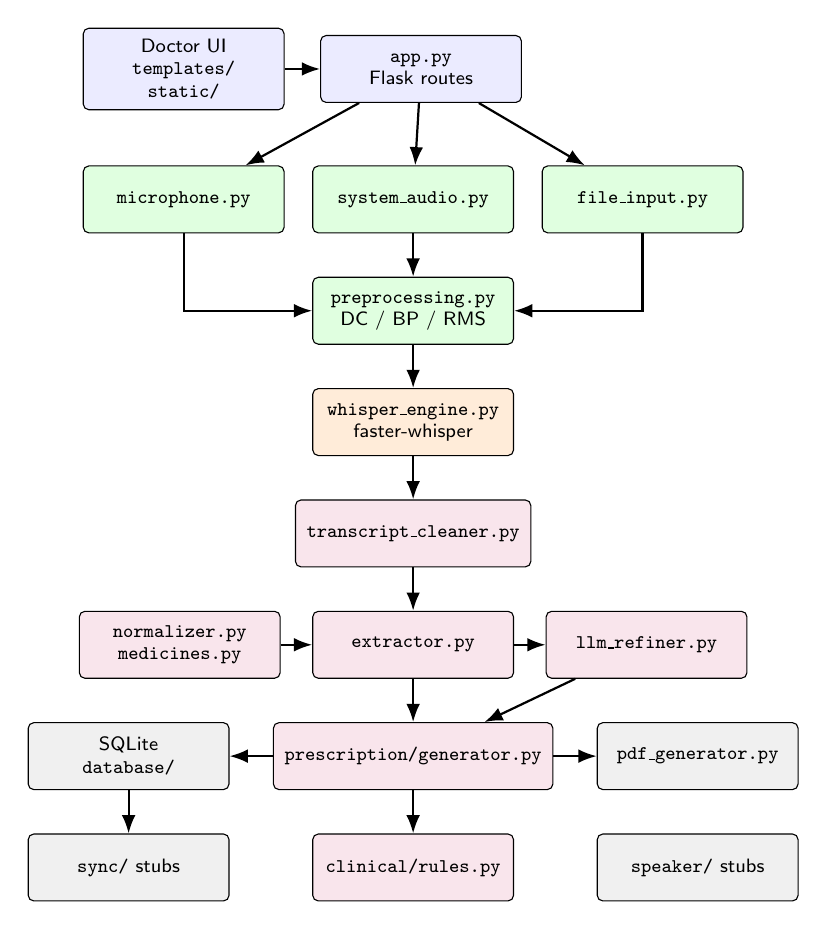
\begin{tikzpicture}[
  font=\scriptsize\sffamily,
  box/.style={draw, rounded corners=2pt, align=center, inner sep=4pt, minimum width=2.55cm, minimum height=0.85cm},
  ui/.style={box, fill=blue!8},
  audio/.style={box, fill=green!12},
  asr/.style={box, fill=orange!15},
  nlp/.style={box, fill=purple!10},
  store/.style={box, fill=gray!12},
  arr/.style={-{Latex}, thick}
]
\node[ui] (ui) {Doctor UI\\ \texttt{templates/}\\ \texttt{static/}};
\node[ui, right=0.45cm of ui] (app) {\texttt{app.py}\\ Flask routes};
\node[audio, below=0.7cm of ui] (mic) {\texttt{microphone.py}};
\node[audio, right=0.35cm of mic] (sys) {\texttt{system\_audio.py}};
\node[audio, right=0.35cm of sys] (file) {\texttt{file\_input.py}};
\node[audio, below=0.55cm of sys] (pre) {\texttt{preprocessing.py}\\ DC / BP / RMS};
\node[asr, below=0.55cm of pre] (wh) {\texttt{whisper\_engine.py}\\ faster-whisper};
\node[nlp, below=0.55cm of wh] (cl) {\texttt{transcript\_cleaner.py}};
\node[nlp, below=0.55cm of cl] (ex) {\texttt{extractor.py}};
\node[nlp, left=0.4cm of ex] (no) {\texttt{normalizer.py}\\ \texttt{medicines.py}};
\node[nlp, right=0.4cm of ex] (llm) {\texttt{llm\_refiner.py}};
\node[nlp, below=0.55cm of ex] (gen) {\texttt{prescription/generator.py}};
\node[nlp, below=0.55cm of gen] (rules) {\texttt{clinical/rules.py}};
\node[store, left=0.55cm of gen] (db) {SQLite\\ \texttt{database/}};
\node[store, right=0.55cm of gen] (pdf) {\texttt{pdf\_generator.py}};
\node[store, below=0.55cm of db] (sync) {\texttt{sync/} stubs};
\node[store, below=0.55cm of pdf] (spk) {\texttt{speaker/} stubs};

\draw[arr] (ui) -- (app);
\draw[arr] (app) -- (mic);
\draw[arr] (app) -- (sys);
\draw[arr] (app) -- (file);
\draw[arr] (mic.south) |- (pre.west);
\draw[arr] (sys) -- (pre);
\draw[arr] (file.south) |- (pre.east);
\draw[arr] (pre) -- (wh);
\draw[arr] (wh) -- (cl);
\draw[arr] (cl) -- (ex);
\draw[arr] (no) -- (ex);
\draw[arr] (ex) -- (llm);
\draw[arr] (llm) -- (gen);
\draw[arr] (ex) -- (gen);
\draw[arr] (gen) -- (rules);
\draw[arr] (gen) -- (db);
\draw[arr] (gen) -- (pdf);
\draw[arr] (db) -- (sync);
\end{tikzpicture}
\caption{Workspace file dependencies and runtime data flow. Speaker matching and cloud sync modules exist as phase stubs and do not currently alter the prescription path.}
\label{fig:arch}
\end{figure}

\subsection{Runtime interaction}
A typical microphone consultation proceeds as follows.
\begin{enumerate}[leftmargin=1.4em]
  \item \texttt{POST /api/mic/start} opens a \texttt{sounddevice.InputStream} with adaptive sample-rate/channel negotiation.
  \item \texttt{POST /api/mic/stop} concatenates frames, downmixes, resamples to 16\,kHz mono PCM, then calls \texttt{asr.transcription.transcribe\_audio}.
  \item Preprocessing writes a temporary WAV; Whisper returns text, language, and timestamped segments; \texttt{clean()} rewrites the transcript string.
  \item The UI posts the transcript onto a consultation via \texttt{/api/consultations/<id>/transcript}.
  \item \texttt{POST .../prescription/generate} invokes \texttt{generate\_from\_transcript}, \texttt{validate\_prescription}, and \texttt{db.save\_prescription} with status \texttt{draft}.
  \item The doctor edits and confirms (\texttt{/api/prescriptions/<id>/confirm}); PDF bytes are streamed from ReportLab.
\end{enumerate}

\subsection{Configuration surface}
\texttt{config.py} centralizes paths (\texttt{data/database.sqlite}), Raspberry~Pi detection (\texttt{/proc/device-tree/model} or \texttt{EMB\_FORCE\_PI}), ASR backend selection (\texttt{auto} prefers faster-whisper), beam size (1 on Pi, 5 on desktop), and the LLM registry (paths, RAM estimates, CPU threads, $T=0$, $n_{\text{ctx}}=2048$, $n_{\text{max}}=512$). System loopback is disabled by default on Pi because \texttt{soundcard} depends on a desktop audio server.

% ===========================================================================
\section{Core Methodology and Mathematical Formulation}

\subsection{Audio acquisition and resampling}
Microphone capture (\texttt{audio/microphone.py}) attempts configurations
\[
  (f_s, C) \in \bigl\{(16\,\text{kHz},1),\ (16\,\text{kHz},C_{\text{dev}}),\ (f_{\text{nat}},1),\ (f_{\text{nat}},C_{\text{dev}}),\ (44.1\,\text{kHz},2),\ (48\,\text{kHz},2)\bigr\}
\]
until PortAudio accepts a stream. After stop, stereo frames are downmixed
\begin{equation}
  x[n] = \frac{1}{C}\sum_{c=1}^{C} x_c[n].
\end{equation}
If the capture rate $f_{\text{cap}} \neq 16\,\text{kHz}$, polyphase resampling (\texttt{scipy.signal.resample\_poly}) converts with integer factors $L=16000/g$ and $M=f_{\text{cap}}/g$ where $g=\gcd(16000,f_{\text{cap}})$. Samples are clipped to $[-1,1]$ and quantized to 16-bit PCM.

\subsection{Preprocessing: DC, bandpass, RMS}
Let $x \in \mathbb{R}^{N}$ be the mono waveform in $[-1,1]$. \texttt{audio/preprocessing.py} computes
\begin{align}
  \tilde{x}[n] &= x[n] - \bar{x}, \qquad \bar{x}=\frac{1}{N}\sum_{n=1}^{N} x[n], \\
  y &= \operatorname{SOSFILT}\bigl(\operatorname{Butter}(K{=}5,\ [f_L,f_H],\ \text{band})\bigr)(\tilde{x}), \\
  \operatorname{RMS}(y) &= \sqrt{\frac{1}{N}\sum_{n} y[n]^2}, \\
  z[n] &= \operatorname{clip}\!\left(y[n]\cdot\frac{\rho^\star}{\operatorname{RMS}(y)},\ -1,\ 1\right),\quad \rho^\star=0.08.
\end{align}
Cut-offs are $f_L=100\,\text{Hz}$ and $f_H=\min(8000, f_s/2-1)$\,Hz, removing 50/60\,Hz hum while retaining speech. Target RMS $\rho^\star \approx -18\,\text{dBFS}$ reduces Whisper VAD false negatives on quiet Bluetooth mics. On failure the original path is returned unchanged.

A dedicated VAD module (\texttt{audio/vad.py}) is still a stub returning a single $[0,T]$ segment; production VAD currently comes from faster-whisper's \texttt{vad\_filter=True}.

\subsection{Clinical ASR}
Let $\mathcal{M}_s$ be a Whisper encoder--decoder of size $s\in\{\text{base},\text{small},\text{medium}\}$, cached under a process-wide lock. Decoding uses temperature $T_{\text{ASR}}=0$ and beam width $B$ (\texttt{ASR\_BEAM\_SIZE}). The clinical initial prompt $p_{\text{clin}}$ (up to Whisper's $\approx 224$ prompt tokens) biases the first-token distribution toward formulary spellings:
\begin{equation}
  \hat{w}_{1:L} = \arg\max_{w_{1:L}} \sum_{t=1}^{L} \log P_{\mathcal{M}_s}\bigl(w_t \mid w_{<t},\, p_{\text{clin}},\, \text{audio}\bigr).
\end{equation}
faster-whisper additionally exposes per-segment average log-probability as a confidence proxy. Local CTranslate2 checkpoints under \texttt{models/whisper/faster-whisper-*} enable fully offline loads.

\subsection{Transcript cleaning}
\texttt{clinical/transcript\_cleaner.clean} is an ordered cascade of idempotent substitutions $\tau_5\circ\tau_4\circ\tau_3\circ\tau_2\circ\tau_1$:
\begin{enumerate}[leftmargin=1.4em]
  \item Spoken numerals $\rightarrow$ digits (compound phrases first: ``5 hundred'' $\mapsto$ 500).
  \item Long-form units $\rightarrow$ \texttt{mg}, \texttt{ml}, \texttt{mcg}, \texttt{IU}.
  \item Spoken/dotted frequencies $\rightarrow$ \texttt{OD}/\texttt{BD}/\texttt{TID}/\texttt{QID}/\texttt{SOS}/\texttt{STAT}.
  \item Known ASR splits (e.g.\ \texttt{augment in} $\mapsto$ Augmentin; spaced \texttt{H B A 1 C} $\mapsto$ HbA1c).
  \item Punctuation injection at duration--drug boundaries to aid clause isolation.
\end{enumerate}

\subsection{Entity extraction}
\texttt{clinical/extractor.extract} returns the prescription-aligned dict
\[
  E = (\text{complaints},\ \text{diagnosis},\ \text{medications},\ \text{investigations},\ \text{advice},\ \text{follow\_up},\ \text{doctor\_notes}).
\]
Symptom and disease lists are sorted longest-first so ``chest pain'' matches before ``pain''. Complaint duration is intentionally empty on the formal draft. Diagnosis uses marker windows of 120 characters plus a fallback keyword scan.

Medication candidates are produced by three scanners: (1)~catalogue regex over \texttt{COMMON\_MEDICINES} keys, (2)~capitalized-name + dose pattern, (3)~verb/form-prefix pattern. For a match span $[s,e]$, clause isolation splits the enclosing sentence on conjunctions so frequency/duration attach to the correct drug. A negation detector drops clauses containing ``avoid'', ``do not take'', ``stop'', ``contraindicated'', etc.

Frequency normalization is a priority list of regexes $\{(r_i, c_i)\}$ mapping Indian numeric schemes and Latin abbreviations onto canonical labels:
\begin{equation}
  F(t) = c_{i^\star},\qquad i^\star = \min\{ i : r_i \text{ matches } t\}.
\end{equation}
Examples: $1{-}0{-}1 \mapsto$ BD; $1{-}1{-}1 \mapsto$ TID; \texttt{HS} $\mapsto$ OD (at bedtime). Duration uses
\begin{equation}
  D(t) = n \cdot u,\quad n\in\mathbb{N},\ u\in\{\text{day(s)},\text{week(s)},\text{month(s)}\}
\end{equation}
with English number-word inversion. Route $\in\{\text{IV},\text{IM},\text{SC},\text{SL},\text{Topical},\text{Inhaled},\text{Oral}\}$.

\subsection{Phonetic and fuzzy drug matching}
Let $V$ be the formulary (\texttt{COMMON\_MEDICINES}). Exact membership yields confidence $1.0$. Otherwise \texttt{fuzzy\_match\_drug}($t$, $\theta{=}0.65$) scores each name $v\in V$:
\begin{align}
  r(t,v) &= \operatorname{SequenceMatcher}(t,v), \\
  \delta_{\text{sx}} &= \mathbf{1}[\operatorname{Soundex}(t)=\operatorname{Soundex}(v)], \\
  \delta_{\text{ph}} &= \mathbf{1}[\phi(t)=\phi(v)], \\
  s(t,v) &= \min\bigl(1,\ r + 0.22\,\delta_{\text{sx}}\delta_{\text{ph}} + 0.12(\delta_{\text{sx}}\oplus\delta_{\text{ph}})\bigr),
\end{align}
with a prefix bonus $s \leftarrow \max(s, 0.88)$ when $v$ starts with $t$ and $|t|\ge 4$ (e.g.\ \texttt{amoxi}$\rightarrow$amoxicillin). Accept if $\max_v s \ge \theta$; flag \texttt{needs\_review} if $s<0.80$. Tokens in \texttt{NON\_MEDICINAL\_WORDS} are rejected immediately.

The medical phonetic key $\phi$ (function \texttt{phonetic\_key}) lowercases, strips non-letters, applies homophone maps (ph$\rightarrow$f, th$\rightarrow$t, c/k/q unification, w$\rightarrow$v, \ldots), preserves the first character, deletes inner vowels, and collapses repeated consonants to length $\le 8$. Soundex uses the standard digit mapping after initial K/Q$\rightarrow$C and PH$\rightarrow$F. Suffix morphology (\texttt{cillin}, \texttt{prazole}, \texttt{sartan}, \ldots) admits novel but drug-like tokens at confidence $0.70$.

\texttt{normalize\_entities} rewrites medication names to catalog generics (or title case), attaches category metadata, and fills missing route/instructions via \texttt{get\_route\_and\_instructions}.

\subsection{Local LLM refinement}
When enabled and a GGUF file exists, \texttt{clinical/llm\_refiner.refine} performs one chat completion:
\begin{equation}
  \hat{J} = \operatorname{LLM}\bigl(\text{system}+\text{few-shot},\ \text{draft JSON},\ \text{transcript}_{\le 1200}\bigr),\quad T_{\text{LLM}}=0.
\end{equation}
Greedy decoding ($T=0$) favors deterministic JSON over diversity. Output parsing is three-tier: direct \texttt{json.loads}, balanced-brace extraction, then repair of trailing commas and single quotes. Alias keys (\texttt{drugs}, \texttt{symptoms}, \texttt{review}) are normalized.

Merge $M(E_{\text{draft}}, E_{\text{LLM}})$ is:
\begin{itemize}[leftmargin=1.4em]
  \item \textbf{Complaints, diagnoses, investigations:} set union (LLM order first).
  \item \textbf{Medications:} if the LLM list validates non-empty, it is authoritative; draft drugs are added only when their brand/generic is not already covered (including combo constituents split on ``+'').
  \item \textbf{Advice / follow-up:} LLM if non-empty, else draft.
\end{itemize}
Failures (missing model, parse error, runtime exception) return $E_{\text{draft}}$ unchanged. A re-entrant lock serializes \texttt{llama.cpp} access across threads (\texttt{tests/test\_concurrency.py}).

\subsection{Clinical decision support}
\texttt{validate\_prescription} maps each medication to brand and generic keys and fires set-intersection rules. Let $P, N, A, M, S, Q, C, I$ be the paracetamol, NSAID, anticoagulant/antiplatelet, macrolide, statin, quinolone, corticosteroid, and mineral sets. Representative predicates:
\begin{align}
  |P_{\text{hit}}|>1 &\Rightarrow \text{duplicate paracetamol / hepatic-limit warning}, \\
  |N_{\text{hit}}|>1 &\Rightarrow \text{dual NSAID warning}, \\
  N_{\text{hit}}\neq\emptyset \wedge A_{\text{hit}}\neq\emptyset &\Rightarrow \text{GI bleeding DDI}, \\
  M_{\text{hit}}\neq\emptyset \wedge S_{\text{hit}}\neq\emptyset &\Rightarrow \text{CYP3A4 myopathy DDI}, \\
  Q_{\text{hit}}\neq\emptyset \wedge C_{\text{hit}}\neq\emptyset &\Rightarrow \text{tendon-rupture DDI}, \\
  \text{asthma/COPD}\wedge \text{beta-blocker} &\Rightarrow \text{error-level contraindication}.
\end{align}
Alerts are structured as $\{\text{level}\in\{\text{info},\text{warning},\text{error}\},\ \text{message},\ \text{field}\}$. Empty medication lists short-circuit with a single warning.

\subsection{Prescription state machine}
\texttt{prescription/schema.py} defines statuses $S=\{\text{draft},\text{confirmed},\text{final}\}$ with transition
\begin{equation}
  \text{draft}\ \xrightarrow{\text{doctor confirm}}\ \text{confirmed}\ \rightarrow\ \text{final}.
\end{equation}
\texttt{new\_prescription} stamps UTC \texttt{created\_at} and a \texttt{CONS-XXXXXXXX} identifier. Confirmation in \texttt{app.py} is an explicit POST; the model never auto-promotes drafts.

\subsection{Persistence}
SQLite (WAL, foreign keys on) stores doctors, patients, consultations, transcripts (\texttt{segments\_json}), prescriptions (\texttt{data\_json}), and \texttt{sync\_queue}. IDs are \texttt{DOC-}/\texttt{PAT-}/\texttt{CONS-} plus eight hex characters. Default seed rows \texttt{DOC-001} and \texttt{PAT-001} enable first-run demos.

Speaker embedding cosine matching
\begin{equation}
  \operatorname{sim}(u,v)=\frac{u^\top v}{\|u\|_2\|v\|_2}
\end{equation}
is specified in \texttt{Plan.md} but \texttt{speaker/enrollment.py}, \texttt{diarization.py}, and \texttt{matcher.py} currently return placeholders and do not filter ASR segments.

% ===========================================================================
\section{Implementation Details and Technical Stack}

\subsection{Primary libraries}
Table~\ref{tab:stack} summarizes the runtime stack. Desktop \texttt{requirements.txt} uses OpenAI Whisper and \texttt{llama-cpp-python}; Raspberry~Pi \texttt{requirements-pi.txt} prefers faster-whisper, \texttt{av<16}, \texttt{pulsectl}, and an OpenBLAS+NEON build of llama.cpp via \texttt{deploy/pi/setup\_pi.sh}.

\begin{table}[htbp]
\centering
\caption{Technical stack as declared in repository requirement files and modules.}
\label{tab:stack}
\begin{tabular}{@{}llp{7.2cm}@{}}
\toprule
\textbf{Layer} & \textbf{Library} & \textbf{Role} \\
\midrule
Web API / UI & Flask, HTML/JS & Routes in \texttt{app.py}; pages \texttt{consultation.html}, \texttt{prescription.html} \\
Capture & sounddevice, soundcard & Mic callback stream; speaker loopback \\
DSP & NumPy, SciPy & Resample, Butterworth SOS, WAV I/O \\
ASR & faster-whisper / openai-whisper & CTranslate2 \texttt{int8} CPU or PyTorch fallback \\
LLM & llama-cpp-python & GGUF chat completion, CPU, $n_{\text{gpu}}=0$ \\
PDF & ReportLab & Letter-size prescription document \\
DB & sqlite3 & WAL local EHR + outbox table \\
Tests & pytest & Phonetic, clinical, Flask, concurrency, LLM \\
\bottomrule
\end{tabular}
\end{table}

\subsection{Concurrency and caching}
Two locks protect heavy models: \texttt{\_model\_lock} in \texttt{whisper\_engine.py} and \texttt{threading.RLock} in \texttt{llm\_refiner.py}. Whisper models are cached by size; switching LLM keys unloads the previous GGUF to stay within Pi memory. Audio recording state is a process-global dict guarded by a lock---not multi-tenant safe, matching the documented single-local-user assumption.

\subsection{Design patterns}
\begin{itemize}[leftmargin=1.4em]
  \item \textbf{Facade / orchestrator:} \texttt{transcribe\_audio} and \texttt{generate\_from\_transcript} hide multi-step pipelines behind one function.
  \item \textbf{Lazy singleton:} \texttt{load\_model} for both ASR and LLM.
  \item \textbf{Strategy:} \texttt{ASR\_BACKEND} $\in\{\texttt{auto},\texttt{faster-whisper},\texttt{openai-whisper}\}$.
  \item \textbf{Repository:} \texttt{database/repository.py} isolates SQL from Flask.
  \item \textbf{Schema factory:} \texttt{new\_prescription} is the canonical object constructor.
  \item \textbf{Graceful degradation:} missing LLM, failed DSP, or disabled loopback never crash the consultation path.
\end{itemize}

\subsection{Formulary schema}
Each catalog entry is
\[
  \{\texttt{generic},\ \texttt{category},\ \texttt{std\_doses},\ \texttt{route},\ \texttt{instructions}\}.
\]
\texttt{lookup} tries exact key, stripped dosage-form suffix, generic-name equality, then first-token match. Approximate cardinality from \texttt{clinical/medicines.py} is on the order of 487 brand/alias keys spanning analgesics, antimicrobials, GI, respiratory, cardiometabolic, and other Indian outpatient brands.

\subsection{Algorithmic sketch}
Algorithm~\ref{alg:rx} restates the prescription generator.

\begin{algorithm}[htbp]
\caption{Draft prescription from transcript (\texttt{generate\_from\_transcript})}
\label{alg:rx}
\begin{algorithmic}[1]
\REQUIRE transcript $T$, optional \texttt{doctor\_id}, patient dict, LLM key
\STATE $E \leftarrow \textsc{Extract}(T)$ \COMMENT{\texttt{clinical.extractor.extract}}
\STATE $E \leftarrow \textsc{NormalizeEntities}(E)$ \COMMENT{phonetic/fuzzy + route fill}
\IF{\textsc{LlmAvailable}(key)}
\STATE $E \leftarrow \textsc{Refine}(T, E, \textrm{key})$ \COMMENT{single chat completion + merge}
\ENDIF
\STATE strip keys starting with \texttt{\_} from each medication
\STATE $R \leftarrow \textsc{NewPrescription}(E)$
\STATE \textbf{return} $R$ with status \texttt{draft}
\end{algorithmic}
\end{algorithm}

\subsection{Representative implementation fragments}
RMS normalization in \texttt{audio/preprocessing.py}:
\begin{lstlisting}[caption={RMS loudness normalization toward $\rho^\star=0.08$.}]
rms = np.sqrt(np.mean(audio ** 2))
if rms > 1e-6:
    audio = audio * (_TARGET_RMS / rms)
    audio = np.clip(audio, -1.0, 1.0)
\end{lstlisting}

Fuzzy score combination in \texttt{clinical/normalizer.py}:
\begin{lstlisting}[caption={Combined string and phonetic score for drug matching.}]
str_ratio = difflib.SequenceMatcher(None, token_clean, name).ratio()
soundex_match = (token_soundex == item["soundex"]) and bool(token_soundex)
phonetic_match = (token_phon == item["phonetic"]) and bool(token_phon)
combined_score = str_ratio
if soundex_match and phonetic_match:
    combined_score = min(1.0, str_ratio + 0.22)
elif soundex_match or phonetic_match:
    combined_score = min(1.0, str_ratio + 0.12)
\end{lstlisting}

LLM fallback contract in \texttt{clinical/llm\_refiner.py}:
\begin{lstlisting}[caption={Public refine() returns the draft unchanged on any failure.}]
def refine(transcript, draft_entities, model_key=None):
    if target_key == "disabled" or not is_available(target_key):
        return draft_entities
    # load, chat-complete, parse, merge; except: return draft_entities
\end{lstlisting}

% ===========================================================================
\section{System Evaluation and Computational Complexity}

\subsection{Repository evidence}
Quantitative results are taken from committed artefacts, not from new runs on this read-only analysis:
\begin{itemize}[leftmargin=1.4em]
  \item \texttt{tests/benchmark\_50\_results.json} --- 50 transcribed clinical cases spanning ENT, pulmonology, gastroenterology, cardiology, endocrinology, pediatrics, dermatology, orthopedics, neurology, psychiatry, urology, and gynecology, evaluated with the Qwen2.5 1.5B Instruct GGUF refiner on top of dictionary extraction.
  \item \texttt{tests/test\_phonetic\_fuzzy.py} --- Soundex/phonetic invariants, non-medicinal rejection, misspelling recovery (\texttt{parasitamol}$\rightarrow$Paracetamol, \texttt{sitrizine}$\rightarrow$Cetirizine).
  \item \texttt{tests/test\_clinical\_scenarios.py} --- multi-drug Indian brands, chronic HTN+T2DM, distractor phrases (``even if'', ``take rest''), pediatric liquids, 1-0-1/TDS/SOS patterns.
  \item \texttt{tests/test\_concurrency.py} --- three concurrent \texttt{refine} threads without llama.cpp crashes.
  \item \texttt{tests/test\_flask\_routes.py} --- UI branding (``Asclepius Clinical''), allowed Whisper sizes \{base, small, medium\}, CRUD consultation workflow.
\end{itemize}

\subsection{Fifty-case extraction benchmark}
Let medication recall for case $i$ be the fraction of expected drug names recovered (brand or mapped generic), and diagnosis accuracy the fraction of cases in which the expected diagnosis substring appears in extracted diagnoses. From the JSON summary:
\begin{align}
  \text{Medication recall} &= 87.69\% \quad (n=50), \\
  \text{Diagnosis hit rate} &= 96.0\%, \\
  \bar{\tau}_{\text{LLM}} &= 9.55\,\text{s per case}.
\end{align}
Per-case latency in the log ranges from roughly 8--18\,s (e.g.\ case\_01 $17.6$\,s, case\_03 $8.3$\,s), consistent with a single CPU chat completion at 512 max tokens. Case\_03 (asthma inhaler regimen) shows a 33\% medication score, illustrating remaining gaps on combo inhaler and less-catalogued brands---exactly why the UI requires doctor review.

\subsection{Safety-oriented qualitative tests}
The extractor and merger are designed so that ``strictly avoid aspirin and ibuprofen'' does not emit those NSAIDs as active prescriptions; few-shot LLM examples encode the same rule. Non-medicinal tokens are dropped before fuzzy matching. Missing dose/frequency produce CDS info/warning rows rather than invented values.

\subsection{Complexity}
Let $N$ be audio samples, $|T|$ transcript characters, $|V|$ formulary size, $L$ LLM context, and $K$ medications in a draft.

\begin{table}[htbp]
\centering
\caption{Asymptotic cost of principal modules (typical consultation: $|T|\!\ll\!10^4$, $|V|\!\approx\!5\cdot 10^2$, $K\!<\!15$).}
\label{tab:complexity}
\begin{tabular}{@{}llp{6.4cm}@{}}
\toprule
\textbf{Module} & \textbf{Time} & \textbf{Space / notes} \\
\midrule
Mic downsample & $O(N)$ & $O(N)$ float32 frames \\
Butterworth SOS + RMS & $O(K_{\text{filt}} N)$ & $K_{\text{filt}}=5$; temp WAV \\
Whisper (faster-whisper) & $\approx O(T_{\text{speech}})$ & Cached weights; VAD skips silence \\
\texttt{clean()} & $O(|T|)$ & Constant number of regex passes \\
Catalogue/med regexes & $O(|T|)$ after $O(|V|)$ compile & Cached \texttt{\_MED\_NAME\_PATTERN} \\
\texttt{fuzzy\_match\_drug} & $O(|V|\cdot |t|\cdot |v|)$ & SequenceMatcher; $|t|,|v|$ small \\
Symptom/disease scan & $O(|\mathcal{L}|\,|T|)$ & Longest-first lists \\
LLM refine & $O(L \cdot d \cdot \text{layers})$ & Weights $\sim$0.8--2.2\,GB RAM; lock \\
CDS set checks & $O(K\cdot |C|)$ & Class sets $C$ are tiny constants \\
SQLite CRUD & $O(\log n)$ typical B-tree & WAL file on disk \\
PDF build & $O(K)$ flowables & In-memory \texttt{BytesIO} \\
\bottomrule
\end{tabular}
\end{table}

Whisper and GGUF dominate wall-clock time; dictionary extraction is negligible. On Raspberry~Pi~5, beam size 1 and \texttt{int8} compute are the primary latency controls. LLM model swap is $O(1)$ API but $O(\text{weight size})$ I/O.

\subsection{Deployment envelope}
\texttt{download\_models.py} packages faster-whisper \{base $\sim$142\,MB, small $\sim$466\,MB, medium $\sim$1.4\,GB\} and three GGUF checkpoints. \texttt{HOW\_TO\_RUN.txt} documents Bluetooth HSP/HFP (not A2DP) as the Pi microphone path. The Flask server binds \texttt{0.0.0.0:5000} so a laptop on the same LAN can drive the UI.

% ===========================================================================
\section{Conclusion and Future Directions}

\subsection{Achievements}
Asclepius Clinical demonstrates a complete local loop from live or uploaded audio to a structured, CDS-checked prescription draft and printable PDF. The hybrid stack---clinical Whisper priming, deterministic cleaners, a large Indian brand catalog, phonetic fuzzy matching, and an optional edge LLM---addresses the characteristic failure modes of generic ASR in Indian outpatient speech. Empirical logs show high diagnosis recovery and strong medication recall on a 50-case specialty suite, with a hard fallback to dictionary extraction when the LLM is absent or malformed. Architectural honesty is equally important: the doctor remains the authority; status never leaves \texttt{draft} without an explicit confirm API.

\subsection{Constraints}
Speaker enrollment, diarization, and doctor-only segment filtering are stubs; mixed doctor--patient audio is fully transcribed. Offline sync HTTP upload, exponential backoff, and PostgreSQL backends are specified in \texttt{Plan.md} and represented by \texttt{sync\_queue} / \texttt{SyncClient} stubs, not production clients. Security items (authentication, encryption at rest, audit completeness, secret hygiene beyond \texttt{SECRET\_KEY}) remain pre-production. Fuzzy matching can still over- or under-merge lookalike brands; LLM latency of $\sim$10\,s may interrupt very fast clinics. The Flask recorder is single-session. Catalog coverage, while broad, cannot be complete for every regional brand.

\subsection{Prospective extensions}
\begin{enumerate}[leftmargin=1.4em]
  \item Replace speaker stubs with embedding models and cosine-threshold gating, never as a sole safety control.
  \item Integrate Silero/WebRTC VAD in \texttt{audio/vad.py} for segmentation before ASR on long recordings.
  \item Implement outbox processing with idempotency keys, TLS, and exponential backoff $t_i = t_0 2^{i}$ as specified for Phase~11.
  \item Expand CDS to renal dosing, pediatric weight-based calculations, and allergy profiles stored on the patient row.
  \item Add multilingual ASR (Hindi/regional) while keeping the English formulary as the normalization target.
  \item Harden authn/z, encrypted voiceprints, and structured audit events before any multi-user clinic deployment.
\end{enumerate}

The present codebase is already a coherent research and engineering artefact: an edge-first clinical NLP system whose mathematics (DSP, phonetic codes, fuzzy scores, greedy LLM decoding, and rule predicates) are realized in named modules, evaluated on committed benchmarks, and bounded by an explicit human confirmation protocol.

\end{document}
